%!TEX root = ../username.tex
\chapter{Physics of Sound Waves}\label{chapter:theory}

\section{Mathematical Background}\label{section:waveforms}
According to Joseph Fourier, the creator of the Fourier Transform, any periodic signal or sound can be reduced into their individual sine waves, or other waveform types \cite{Broughton_Bryan_2008}. There are five basic periodic waveform types: a sine wave, square wave, sawtooth wave, triangle wave, and pulse wave \cite{Winer_2018}. The pulse wave is a special type of waveform, as it is a non-sinusoidal waveform which includes square waves within it, and is similarly periodic to square waves, but also asymmetrical, but will not be discussed within the scope of this project. The other waveform types repeat in a pattern of motion known as a cycle, and the period is the time length.

In its most basic form, there are three general types of waves \cite{Halliday_Resnick_Walker_2005}.

\begin{enumerate}
	\item Mechanical waves.
	\item Electromagnetic waves.
	\item Matter waves.
\end{enumerate}

Mechanical waves are the most familiar to many, due to its ubiquity; mechanical waves are found as water waves, sound waves, and sonic waves. These waves are known by two key features: a governance by Newton's three laws, and an existence that occurs only within a material medium, such as air or water. Additionally, these waves follow the idea of \textit{simple harmonic motion}, in which the wave oscillates in a specific path, and varies sinusoidally in time, following a sine or cosine function. Electromagnetic waves are the second most familiar type of wave, found in visible and ultraviolet light, x-rays, and radar waves. Unlike mechanical waves, electromagnetic waves do not require any material medium to exist, able to travel through a vacuum at a speed of $c = 299,792,458 \textrm{ } m/s$. Finally, matter waves are the least frequently recognized type of wave, though it is commonly found in technology. These waves work within fundamental particle types, including protons, electrons, atoms, and molecules. 

The speed with which each wave rises and falls is its frequency $f$. If the frequency is too low (less than 20 cycles per second, or 20 Hertz, abbreviated as Hz), little to no noise will be audible by the human ear. If the frequency is too high (generally above 20,000 cycles per second, or 20 kiloHertz, abbreviated kHz), again, few noises besides high-pitched and shrill noises will be audible. The range of human hearing is generally stated as being from 20 cycles per second, with 20 Hertz at the low end to 20,000 cycles per second (20 kHz) at the high end. Older people generally lose the ability to hear the higher frequencies.

For any sine wave, one method of notating the sine wave function is in Equation \ref{eq:physics-sine-wave} \cite{Halliday_Resnick_Walker_2005}, describing a sine wave which oscillates parallel to the y-axes at time \texttt{t}, with the displacement of $y$ at position $x$.

\begin{equation}
	y(x,t) = y_m \sin(k(x + \lambda) - \omega t)
	\label{eq:physics-sine-wave}
\end{equation}

The amplitude of a wave ($y_m$) is the magnitude of the maximum displacement of the wave's crest (peak or trough) from its equilibrium position. As this value is a magnitude, the quantity of amplitude will always be positive, even if it measures the trough of a wave instead of the peak. The phase of wave ($kx - \omega t$) will change linearly with a time \texttt{t}, dependent on the oscillation of the wave. Arbitrarily, as a sine wave oscillates between values of $-1$ and $+1$, the wave's amplitude is at value $-y_m$ and $+y_m$ respectively. Thus, the time-dependent nature of the wave's phase will correspond to the oscillation of the wave, with the amplitude determining the extremeness of the displacement of the wave's crest. The wavelength $\lambda$ of a wave is the distance between repetitions of peaks or troughs, and is parallel to the direction of the wave's travel. Finally, the period of a wave \texttt{T} is the time to move through one full oscillation \cite{Halliday_Resnick_Walker_2005}. Due to the nature of a sine wave to follow the unit circle counterclockwise (discussed more in Subsection \ref{subsection:sine-waves}), the sine wave will begin to repeat when its angle $\theta$ (or argument $k$) is increased by $2\pi$. Thus, we also have Equation \ref{eq:sine-wave-period} which is equivalent to Equation \ref{eq:physics-wavelength}.

\begin{equation}
	k = \frac{2\pi}{\lambda}
	\label{eq:physics-wavelength}
\end{equation}

So, we now have two types of frequency: $\omega$ (angular frequency) and $f$ (temporal frequency). The temporal frequency $f$ of a wave is defined relative to angular frequency $\omega$, as in Equation \ref{eq:physics-freq-eq}. Frequency $f$ is the number of oscillations per unit time, usually measured in Hertz or kiloHertz. Angular frequency is the frequency of an arbitrary sine wave as it moves counterclockwise around the unit circle.

\begin{equation}
	f = \frac{1}{T} = \frac{\omega}{2\pi}
	\label{eq:physics-freq-eq}
\end{equation}

The final way in which we are able to easily study waves is to monitor the wave forms (the shape of the waves) as the waves move left to right. Alternatively, we could also monitor the wave as it oscillates up and down, but the result is the same: either the displacement of the peaks and troughs of an oscillating wave is perpendicular to the direction of travel of the wave, or the direction of travel of an oscillating wave is parallel to the displacement of the crest of the wave \cite{Halliday_Resnick_Walker_2005}. This first type of motion is a \textit{transverse wave}, and the second is a \textit{longitudinal wave}, as in Figure \ref{fig:transverse-wave-longitudinal-wave}. Both wave shapes are also known as \textit{traveling waves} as they travel from one defined point to another.

\begin{figure}[ht]
  \centering
  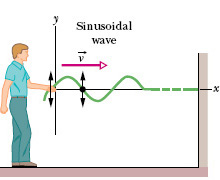
\includegraphics[width=0.5\textwidth]{fig_16_1.jpeg}
  \caption{(a) A single pulse is sent along a stretched string. A typical string element (marked with a dot) moves up once and then down as the pulse passes. The element’s motion is perpendicular to the wave’s direction of travel, so the pulse is a transverse wave. (b) A sinusoidal wave is sent along the string. A typical string element moves up and down continuously as the wave passes. This too is a transverse wave.}\cite{Halliday_Resnick_Walker_2005}
  \label{fig:transverse-wave-longitudinal-wave}
\end{figure}


\subsection{Sine Waves}\label{subsection:sine-waves}
The first of the basic periodic waves is the sine wave, and is the most common type of periodic wave. The sine wave is a signal with only one frequency, and represents the unidimensional motion for any signal with a phase angle that rotates at a constant rate. It is also based on the trigonometric sine function. On the unit circle, the trigonometric sine function of a phase angle $\theta$ is defined as the ratio of the length of the opposite side and the hypotenuse of a right triangle. The unit circle, with a radius of 1, results in the sine function $sin\theta$ being equal to the y-value in Cartesian coordinates, where the hypotenuse of the right triangle that is formed meets the circle, like in Figure \ref{fig:unit-circle}. We can then use this trigonometric sine wave to synthesize a sine wave audio signal. As sine wave is a continuous periodic wave, in which the wave continues to sound until stopped, we must use the sine wave function on the unit circle continuously. Thus, we use the sine function continuously around the unit circle, going counterclockwise. We notice that in the correlation between Figures \ref{fig:basic-sine-wave} and \ref{fig:unit-circle} moving counterclockwise through the unit circle results in the appropriate rise and fall of the sine wave. $\frac{\pi}{2}$ is the highest y-value within the Cartesian plane, and so denotes a peak in the sine wave, while $\frac{3\pi}{2}$ is the lowest, denoting a trough.

\begin{figure}[h]
	\centering
	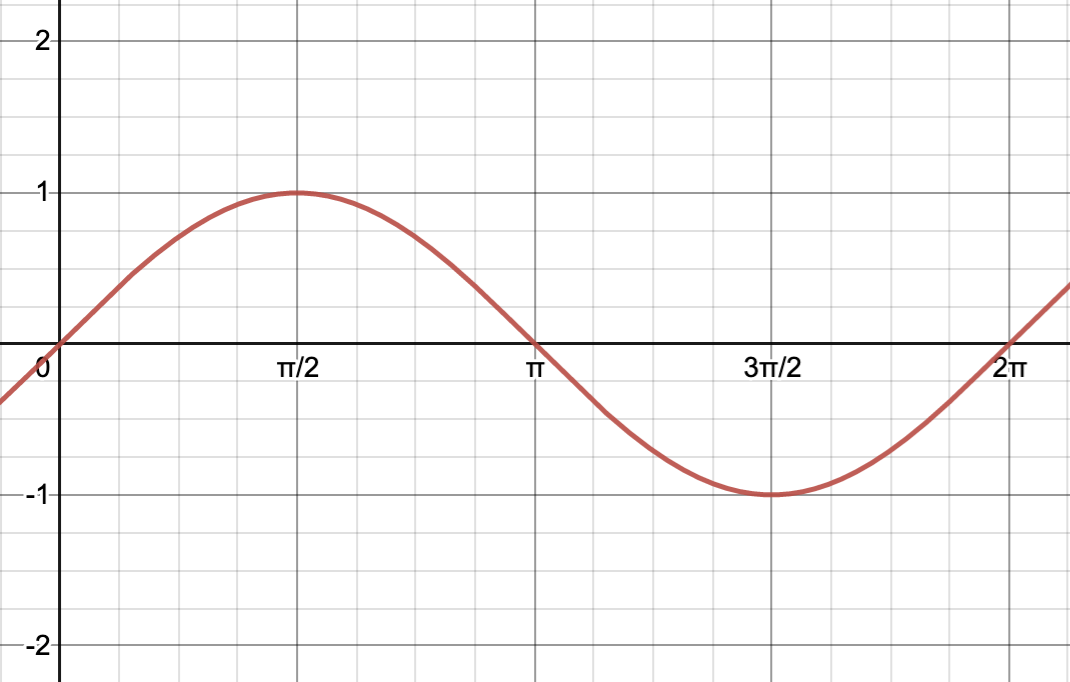
\includegraphics[width=0.5\textwidth]{figures/sine-wave-form.png}
	\caption{A basic sine wave}
	\label{fig:basic-sine-wave}
\end{figure}

\begin{equation}
	y = Asin(B(x + C)) + D
	\label{eq:sine-wave-equation}
\end{equation}

Like with the other periodic waves, sine waves have three important properties: frequency, amplitude, and phase. From the generic function for a sine wave as in Equation \ref{eq:sine-wave-equation}, we are able to compute the various properties. First, \textit{A} is the sine wave's amplitude. This is defined as the height from the center line of the wave to its peak or trough. For our unit sine wave, this value will be 1. Second is the variable \textit{B}, which helps to define the period of the wave, or the distance between one peak and the next, or one trough and the next. With Equation \ref{eq:sine-wave-period}, we see the period is equivalent to taking the total circumference of the unit circle, and dividing it by \textit{B}. Third, the phase shift of a sine wave is denoted by \textit{C}. If the expression is $(x + C)$, then the phase of the sine wave will shift to the left, as the x-value of the wave becomes negative \textit{C}. Otherwise, if the expression is $(x - C)$, then the wave will shift right, with a positive x-value as \textit{C}. Finally, the variable \textit{D} is equivalent to the vertical shift of the wave. This notates the distance that the wave will shift vertically from its unit circle position.

\begin{equation}
	\frac{2\pi}{B}
	\label{eq:sine-wave-period}
\end{equation}

\begin{figure}
	\centering
	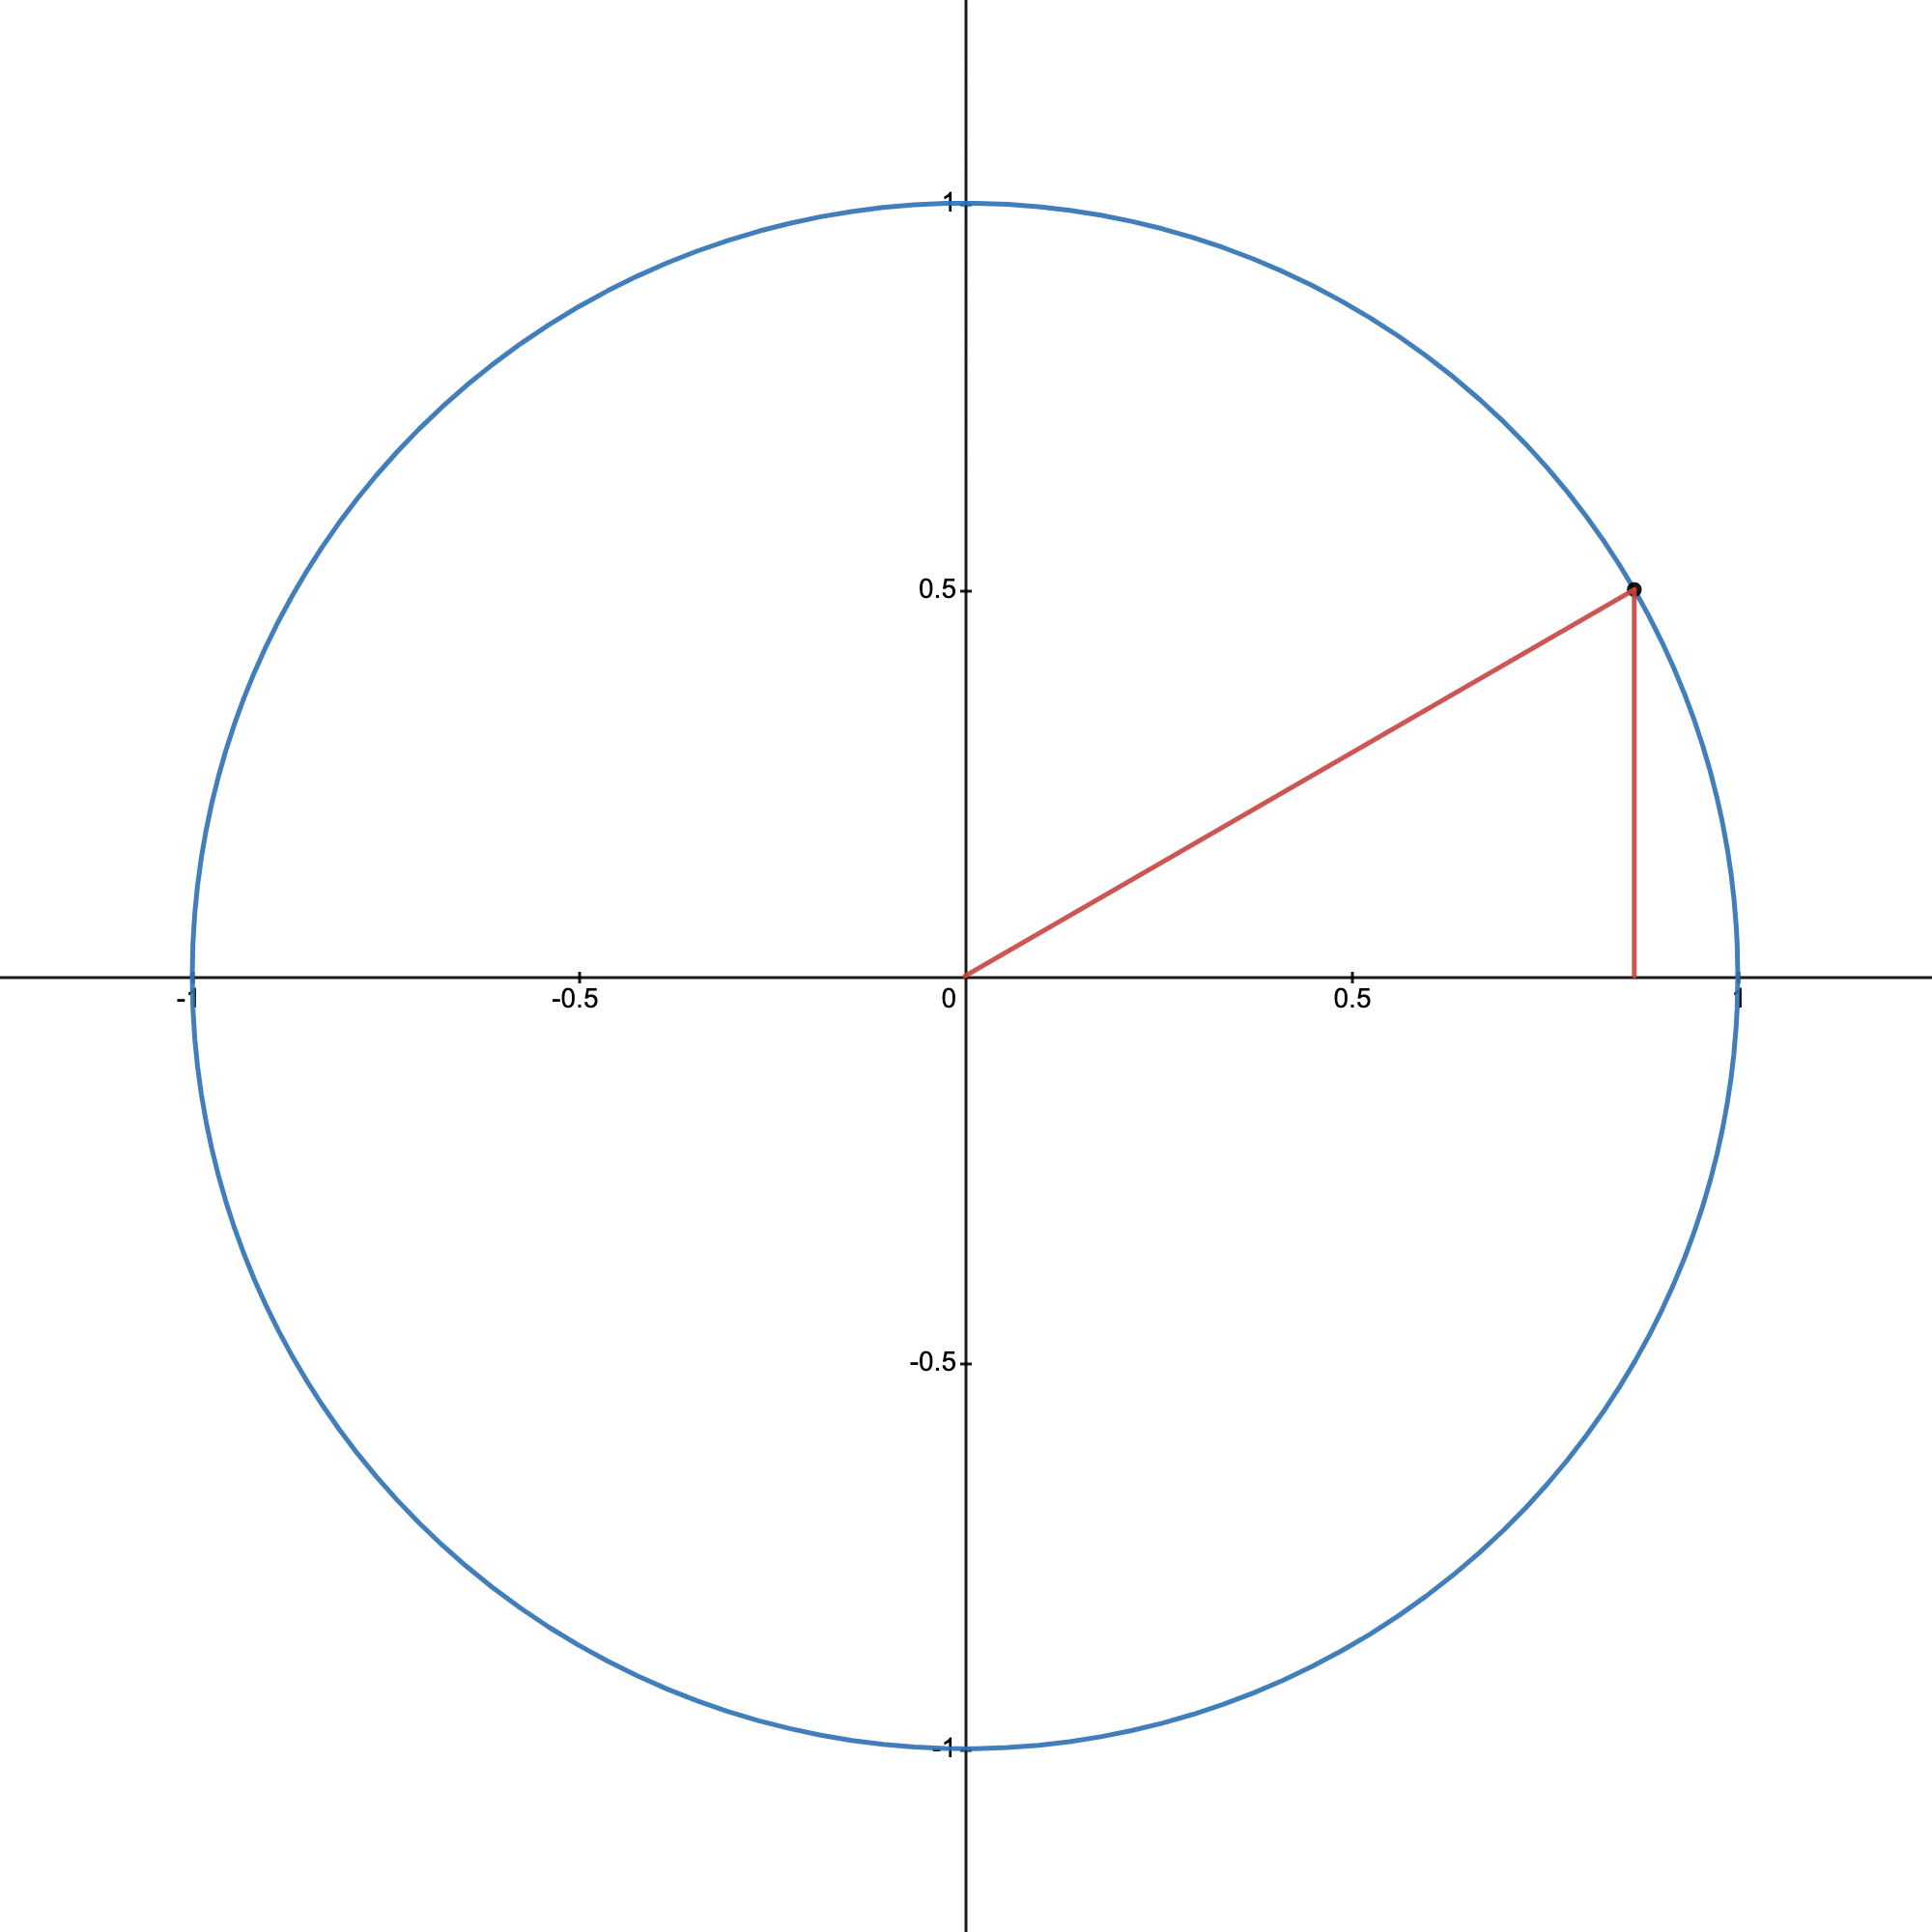
\includegraphics[width=0.5\textwidth]{figures/unit-circle.png}
	\caption{The unit circle}
	\label{fig:unit-circle}
\end{figure}

\subsection{Square Waves}
The square wave is the second of the periodic waveforms, and is a wave in which the frequency oscillates between a single fixed minimum and maximum value \cite{Tarr_2019}. Within the unit circle definition of the square wave, the maximum frequency is positive or negative one, as in Figure \ref{fig:square-wave}. This unit square wave details the ideal square wave, in which the change between minimum and maximum frequency happen instantaneously. An approximation of square waves may be created through the combination of multiple individual harmonics (sine functions). This method of creating an audio signal is known as \textit{additive synthesis}, in which a new timbre or sound is create by adding together periodic waveforms, usually sine waves \cite{Tarr_2019}. 

The square wave is a certain type of pulse wave which allows for a frequency to sound at fixed amplitudes for an arbitrary duration. At its simplest, a square wave can be defined as a sign function of a sinusoidal. A sign function, or a signum function, as in Figure \ref{fig:sign-function}, is an odd mathematical function which extracts the sign of a real number, expressed as $sgn$. Of a real number $x$, it is a piecewise function, defined as in Equation \ref{eq:sgn-function}.

\begin{equation}
	sgn (x): \begin{cases}
		-1 & \textrm{if } x < 0, \\
		0 & \textrm{if } x = 0, \\
		1 & \textrm{if } x > 0
	\end{cases}
	\label{eq:sgn-function}
\end{equation}

\begin{figure}[h]
  \centering
  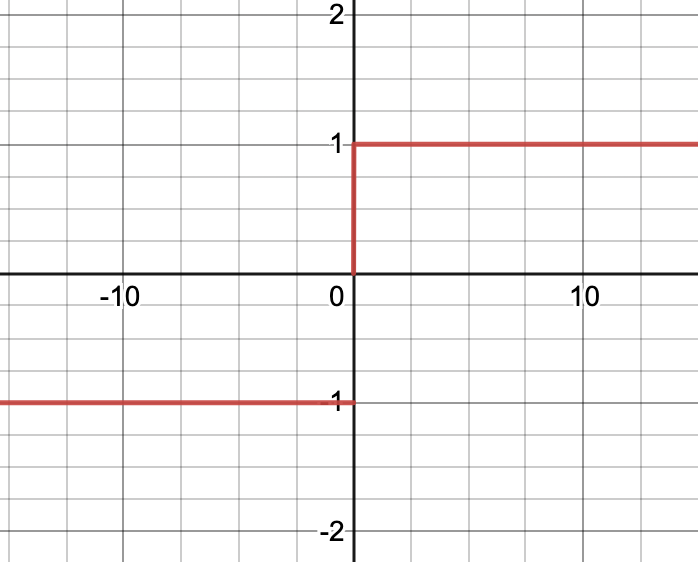
\includegraphics[width=0.5\textwidth]{sign-function.png}
  \caption{A sign function}
  \label{fig:sign-function}
\end{figure}

Thus, we have a square wave equal to Equation \ref{eq:square-wave-function}. The function $x(t)$ will equal 1 when the sinusoidal is positive, -1 when negative, and 0 at the discrete values where the sinusoidal is equivalent to 0.

\begin{align}
	x(t) = sgn(sin2\pi ft)
	\label{eq:square-wave-function}
\end{align} 


\begin{figure}[h]
  \centering
  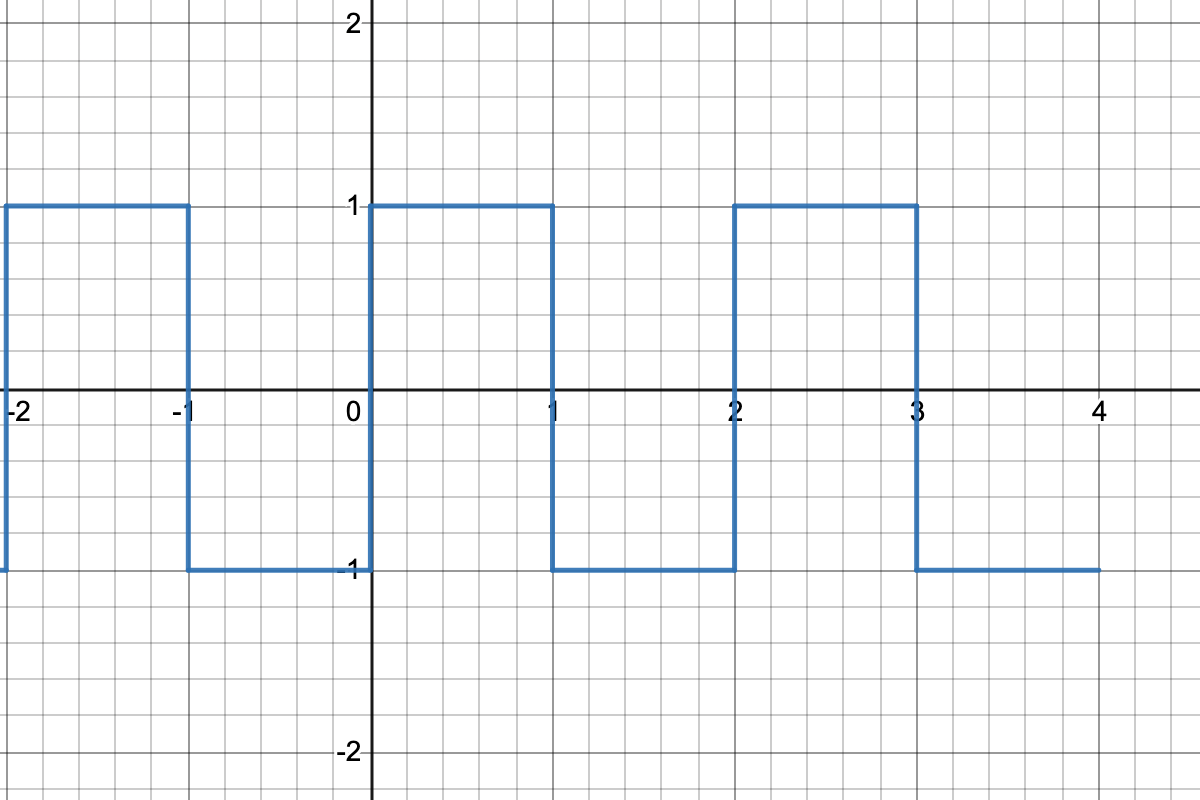
\includegraphics[width=0.3\textwidth]{square-wave.png}
  \caption{A basic square wave}
  \label{fig:square-wave}
\end{figure}

Similar logic to sine waves can be applied to square waves to alter the sound of a square wave. 

\subsection{Sawtooth Waves}
The sawtooth waveform is also a non-sinusoidal wave, which resembles the teeth of a plain-toothed saw. Similar to the square wave, a sawtooth wave will ramp upwards to a peak amplitude height, then sharply drop to its trough, as in Figure \ref{fig:basic-sawtooth-wave}. Then, we are able to take Equation \ref{eq:sawtooth-piecewise-function}, and place it into a periodic function, as in Equation \ref{eq:sawtooth-sinusoidal-function}. For the periodic function, let $frac(x) = t - \lfloor t \rfloor$.

\begin{equation}
	x(t) = t - \lfloor t \rfloor
	\label{eq:sawtooth-piecewise-function}
\end{equation}

\begin{equation}
	S(x) = Afrac(\frac{x}{T} + \phi)
	\label{eq:sawtooth-sinusoidal-function}
\end{equation}

Like with other waveforms, the variable \textit{A} represents the wave's amplitude, and \textit{T} represents the wave's period. The variable $\phi$ denotes the wave's phase, with positive values causing a shift to the left, and negative values a shift to the right. Sawtooth waves are typically created through additive synthesis, much like square waves are, and so we notice that sawtooth waves and square waves have similar periodic equations \cite{Tarr_2019}.

\begin{figure}
  \centering
  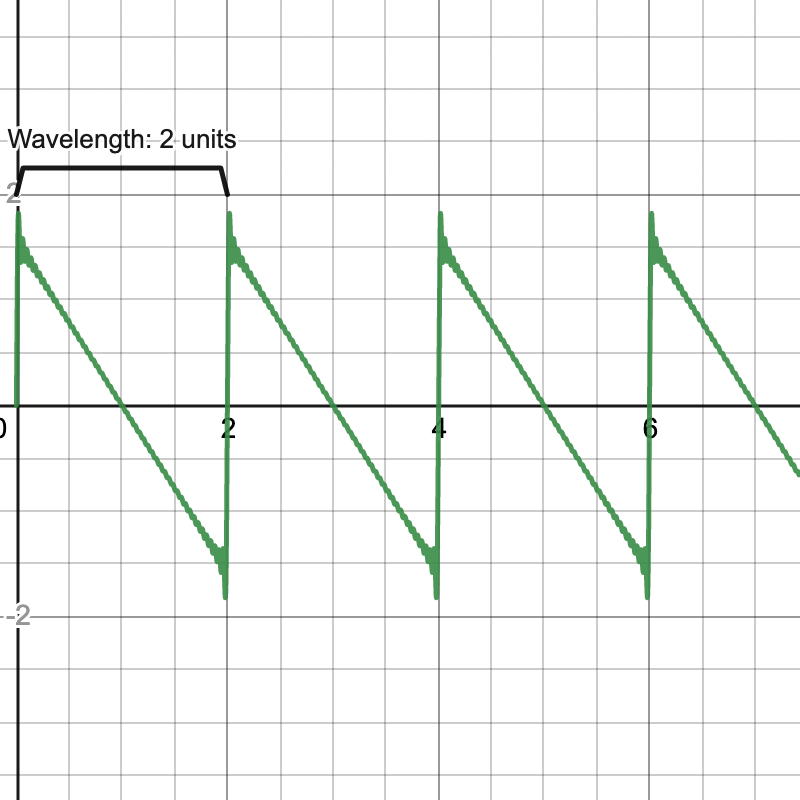
\includegraphics[width=0.5\textwidth]{figures/sawtooth-wave.png}
  \caption{A basic sawtooth wave}
  \label{fig:basic-sawtooth-wave}
\end{figure}


\subsection{Triangle Wave}

A triangle wave is also a non-sinusoidal waveform, named for its triangular shape. Like with square waves, this type of wave only contains odd harmonics, i.e. only containing valid values which are odd numbers.

\begin{equation}
	f(x) = \frac{2}{\pi}sin^{-1}\lceil sin(\pi x) \rceil
	\label{eq:triangle-wave-function}	
\end{equation}

\section{Representing Sound Digitally}

We now understand the physics and mathematics behind sound waves. However, sounds in real life are not composed of simple pure waveforms; sounds in the world around us are made up of multiple harmonics and frequencies layered on top of one another to produce the composite sound which we hear. Sound, like electricity and light, is a form of energy in which molecules in air vibrate and move in a wave pattern. This wave pattern produces the sound waves \cite{Au-Yeung_2021}. Air is able to support multiple sound waves simultaneously, explaining our ability to hear different sounds at the same time. This sound energy is dispersed outwards from the sound source, and will continue to move until the molecules run out of energy, as the energy weakens the further it moves away from the sound source. The sound energy is transferred between molecules, as each molecule moves from an original resting point, transfers energy to another molecule, then returns to its resting point, as in Figure \ref{fig:graphical-rep-vs-physical-sound}. This molecule movement is the oscillation of sound. Molecules become closer together when vibrating, and crowd together in certain places, and thus there are fewer molecules in other places. This visualization of crowds of molecules can be done as a wave, with the peak of a sound wave indicating that there are more molecules together in space (compression of air molecules), and the trough of a sound wave indicating there are fewer molecules (rarefaction) \cite{Toft_2020}. Typically, sound is visualized in a graphical format, with peaks and troughs to a wave rather than drawings showing the compression and rarefaction of air molecules. 

\begin{figure}
  \centering
  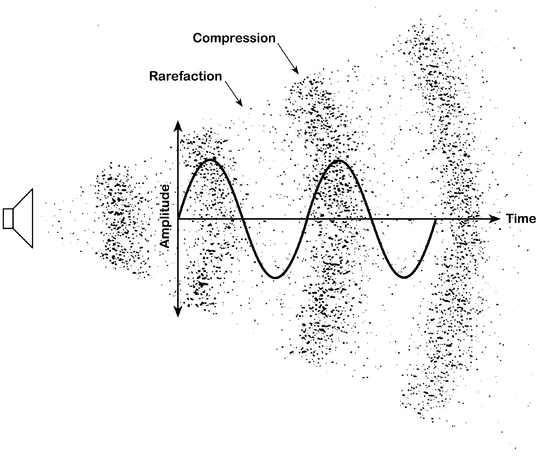
\includegraphics[width=0.4\textwidth]{graphical-rep-vs-physical-sound.jpeg}
  \caption{A graphical representation of sound, vs its physical phenomenon}\cite{Toft_2020}
  \label{fig:graphical-rep-vs-physical-sound}
\end{figure}

Through this periodic nature of waves, the repetitions create what we will recognize to be musical sound, but lacking the specific tonality and timbral qualities of specific instruments. Musical instruments generate a composite set of frequencies, arranged as a layered set of harmonics above the fundamental frequency (the first frequency which is played, typically the lowest). Thus, the fundamental frequency will be the pitch of the note, and the additional harmonics (also known as overtones) will lie above this pitch and add the tonality or timbre of the note \cite{Toft_2020}. This is what differentiates pure sound waveforms from notes generated from musical instruments, as pure sound waveforms all have pitch, but lack specific timbral quality.\footnote{This is what gives pure sound waveforms their name, ``pure tones,'' as each of these waveforms has pitch but no timbre.} Another factor which dictates what a sound wave will be perceived as is the amplitude of a wave. The wave's amplitude is the distance from the middle of a wave to its crest (peak or trough). Amplitude is also known as the sound's volume, as adjusting the amplitude of a wave will result in a louder sound, and will be further discussed in Section \ref{section:manip-waves}.

To get from an analog sound wave to a digital sound signal, we must sample the continuous analog wave into its digital representation. While an audio signal or sound is a continuous set of values, which are able to be displayed on an oscilloscope (a tool to show oscillations) as a waveform, the digital ``signal'' is a series of numbers, representing various discrete values from the continuous wave. These numbers will represent the values of an audio signal at specific points in time, and are known as \textit{samples} \cite{Russ_2012}. The sampling process to convert from analog (physical) waves to a digital signal involves three steps:

\begin{enumerate}
	\item The audio signal is ``sampled.''
	\item The sample value is converted into a number.
	\item This number is presented at an output port.
\end{enumerate}

The process of sampling will typically produce numbers which are an incomplete representation of the original audio sound, but through careful sampling, this amount of incompleteness can be made insignificant. This same process can be reversed to convert from a digital signal to an analog one, and is known as ``sample replay.'' Sample replay also has three stages and serves as the basis for digital synthesizers, as the conversion from digital signal to analog wave produces the sound that is heard:

\begin{enumerate}
	\item A number is presented to an input port.
	\item This number is converted into an analog signal.
	\item The analog value forms part of an audio signal.
\end{enumerate}

Analog sound exists in two dimensions: time (a period of each wavelength) and space (the displacement of each waveform from the atmospheric pressure). So it makes sense that to convert from analog audio to digital signals, we use these two dimensions: time (\textit{sample rate}) and space (\textit{bit depth}). 

\textit{Sample rate}, or \textit{sample frequency}, is the number of samples which are captured per period (which is commonly measured in Hertz). Typically, digital audio samples of analog audio waves are taken at a rate of 8,000 times per second, or more \cite{Zjalic_2021}. Occasionally, a sound will be sampled that is at a frequency rate higher than 8,000 and the system doing the sampling is unable to identify two points on the waveform to understand the period. Harry Nyquist (1879-1976) was a Swedish physicist and electrical engineer who solved this problem, through the \textit{Nyquist frequency} (or \textit{folding frequency}). Nyquist discovered that in order for an analog audio wave to be accurately represented by a digital signal, and thus also the system which is sampling the audio wave, the wave must be sampled at least twice per wavelength, known as the \textit{Nyquist Theorem} \cite{Zjalic_2021} and visualized in Figure \ref{fig:nyquist-sampling-theorem}. Thus, for a given sample rate, the highest frequency within a system cannot exceed half this sample rate. In other words, the Nyquist frequency is the frequency at 50\% of the sample rate. Otherwise, for a frequency which does not satisfy the requirements for the Nyquist Theorem, a phenomenon called ``aliasing'' would occur, in which signals that exceed half the sample rate are misrepresented as ``alias signals.'' An ``anti-aliasing'' filter would then typically be applied to the signal before sampling occurs, to act as a low-pass filter with a cut-off at the Nyquist frequency.


\begin{figure}[ht]
  \centering
  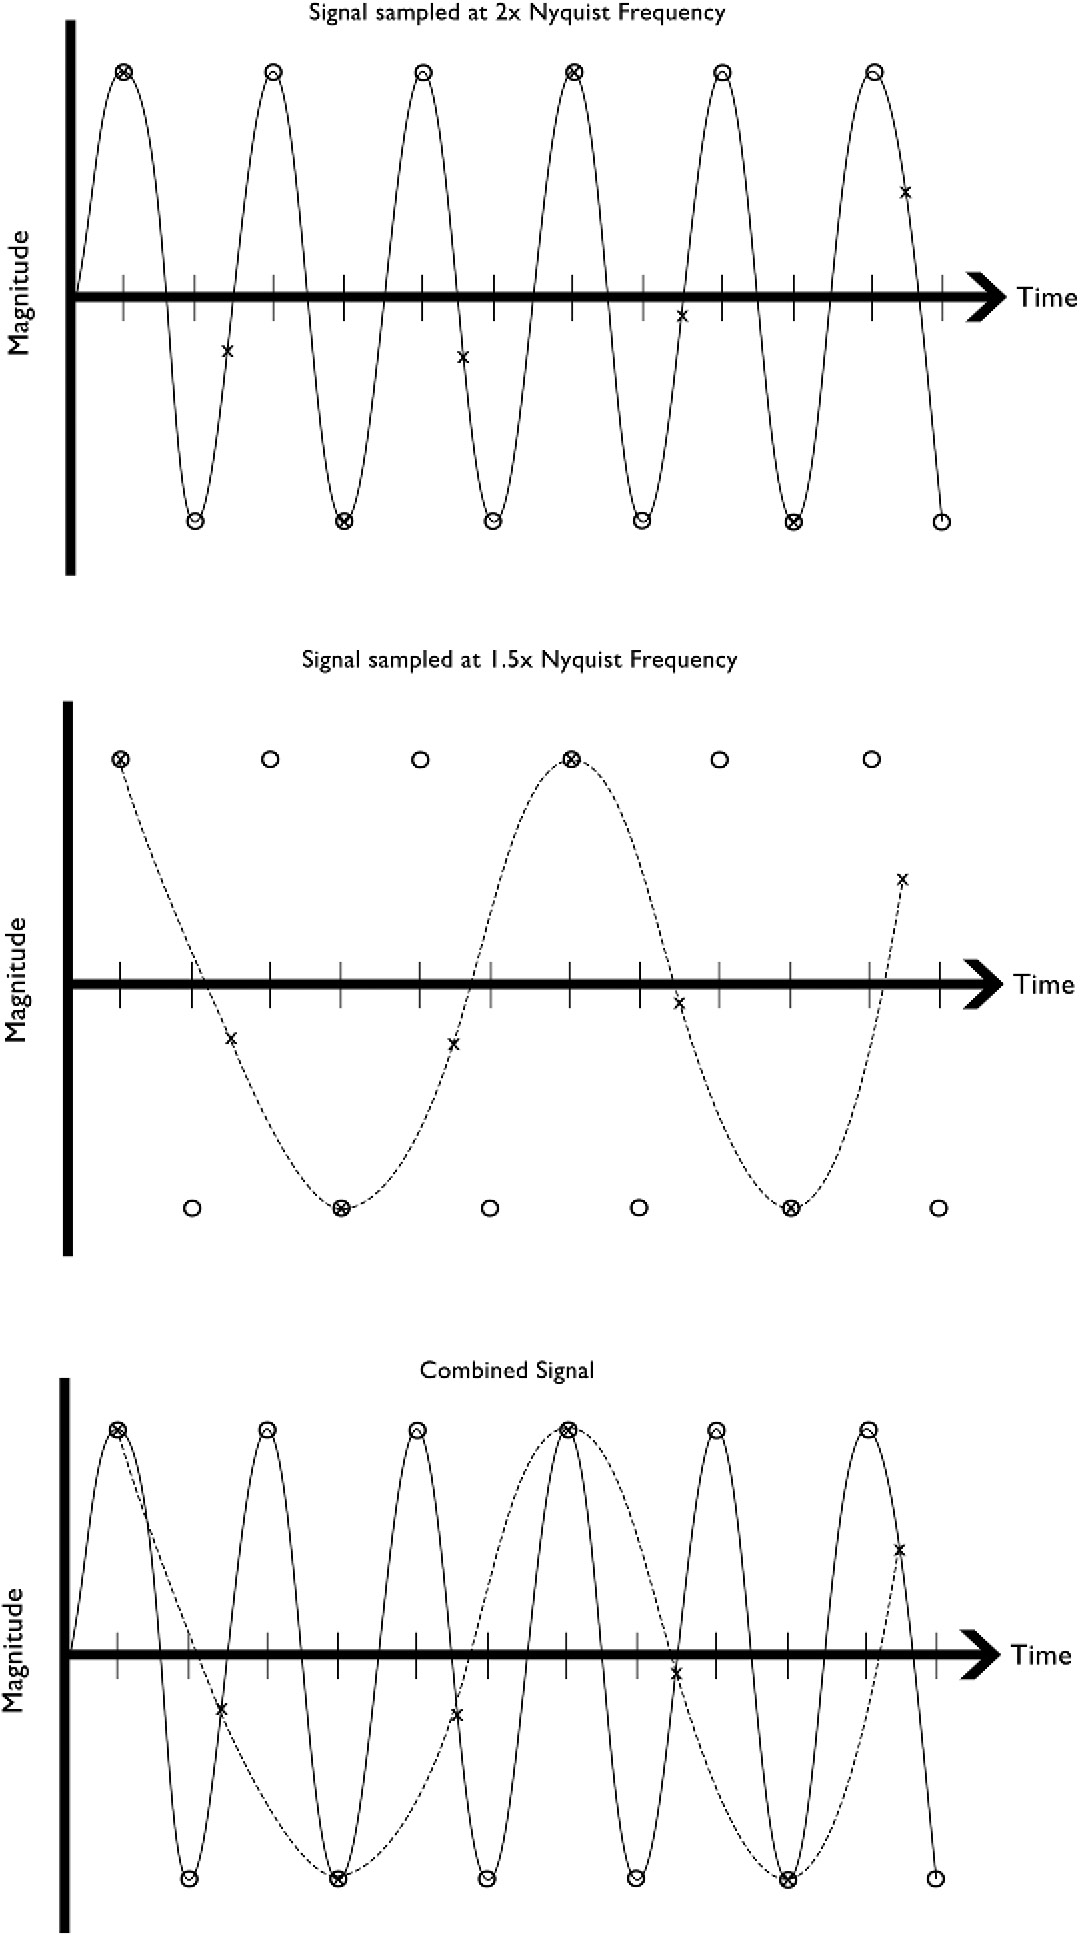
\includegraphics[width=0.5\textwidth]{nyquist-sampling-thoerem.jpeg}
  \caption{The Nyquist sampling theorem visualised. Upper: Signal sampled at 2x Nyquist frequency, Middle: Signal sampled at 1.5x Nyquist frequency (and thus aliasing and not a true representation of the original signal), Bottom: Signal containing both accurate and aliasing components}\cite{Zjalic_2021}
  \label{fig:nyquist-sampling-theorem}
\end{figure}


\textit{Bit depth} is defined as the discrete values which are available within the digital system, representing the magnitude of a continuous electrical signal \cite{Zjalic_2021}, in the form $log_2{x}$. These levels can become exponentially large, and so \textit{quantization} is used, to process data from a broad range into values within a smaller range. It will convert the levels of a continuous analog signal, as the signal after sampling is still in the analog domain, into binary digits (bits). Using bits will allow us to be able to manipulate and store audio data digitally. After sampling the amplitude of an analog audio wave at various precise intervals, we are able to output this amplitude level in its equivalent in bits, which represent the originally sampled amplitude level, known as \textit{bit rates}. The bit ``rate'' can then be defined as the amount of data stored or transmitted per second of time, or in Equation \ref{eq:bit-rate}, measured in kbps \cite{Zjalic_2021}. In general, the higher the value of the bit rate, the higher the quality of the audio data that is stored, since there is more data to represent the captured sound available.

\begin{equation}
	\textrm{bit rate (bits per second)} = \textrm{sample rate (Hz) x } \textrm{bit depth x } \textrm{number of channels}
	\label{eq:bit-rate}	
\end{equation}

From our original three stages of converting analog sound to digital signals, we can now specify the processes which occur in each stage \cite{Huber_Runstein_2018}. Upon playback, the bits are then converted back into analog amplitude values, at precise intervals in time, allowing for the originally recorded amplitude values to be re-created, processed, and played back \cite{Huber_Runstein_2018}. 

\begin{enumerate}
	\item Sampling analog audio wave amplitude levels at precise intervals in time.
	\item Converting these samples into the digital bit value (typically a 16-bit length), which most accurately represents the amplitude levels.
	\item Storing these sample equivalents (the bit values) within digital memory.
\end{enumerate}


\section{Manipulating Sound Waves}\label{section:manip-waves}
As previously mentioned in Section \ref{section:modular-synth-what-is}, modular synthesis involves sending an audio signal through patches or modules in a linear format to achieve the desired sound output changes. To explain how these changes occur to a sound wave, we arbitrarily choose the simple sine wave as an example, as in Figure \ref{fig:sine-wave-period-amplitude}. Sine waves are a waveform which is a function of time \texttt{t}

\begin{figure}[h]
	\centering
	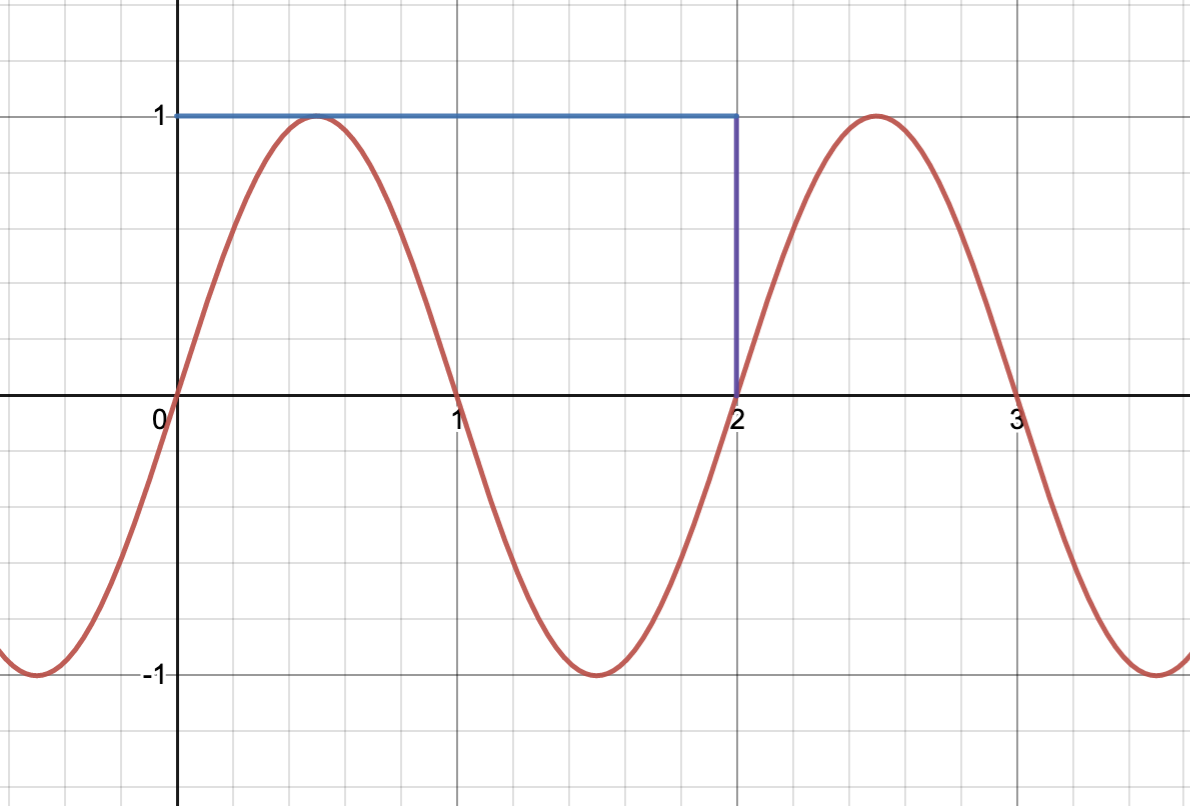
\includegraphics[width=0.5\textwidth]{figures/sine-wave-period-amplitude.png}
	\caption{A basic sine wave, with period demarcated in blue, and amplitude in purple}
	\label{fig:sine-wave-period-amplitude}
\end{figure}

\begin{equation}\label{eq:full-sine-wave-equation}
	y(t) = A \sin(2\pi ft + \varphi)
\end{equation}

with variables $A$, $\varphi$. $A$ is the wave's amplitude, which determines the peak deviation from zero. The frequency is $f$, and $\varphi$ is the wave's phase, which specifies (in radians) where in its cycle the wave's oscillation is at time $t$ \cite{Kirk_Hunt_2013}. When $\varphi$ is not equal to zero, the wave itself will appear to be shifted by the value equal to $\varphi$, which is known as a wave's \say{phase shift.} A negative value will represent a delay in sound, while a positive value will represent an advance in the heard sound.

Thus, there are three primary options when manipulating audio (or a simple waveform); amplitude, frequency, and phase can all be modified at various points to affect the audio output. The first, amplitude, will determine the volume of the wave's sound. The larger the distance between zero and the wave's peak, the louder the human ear will perceive the sound to be\cite{Zjalic_2021}. In Figure \ref{fig:sine-wave-period-amplitude}, amplitude is colored purple, and we see it has a value of 1 (the default value of amplitude of a sine wave from the unit circle), as $A$ does in Equation \ref{eq:full-sine-wave-equation}. By changing the value of $A$ to either $\frac{1}{2}$, or $2$, the peak of the wave will change accordingly, becoming larger or smaller depending on the set value of $A$. This change is reflected in the sound we can hear, as like in Figure \ref{fig:half-sized-sine-wave} and Equation \ref{eq:half-sized-sine-wave}, the volume of this sine wave is halved. Thus, volume ranges can be between soft (at a barely audible \textit{pianissimo}) with an amplitude $A = \frac{1}{2}$, or loud (\textit{fortissimo}), with $A = 4$, for instance.

\begin{equation}\label{eq:half-sized-sine-wave}
	y(t) = \frac{1}{2} \sin(\omega t + \varphi)
\end{equation}

\begin{figure}[h]
	\centering
	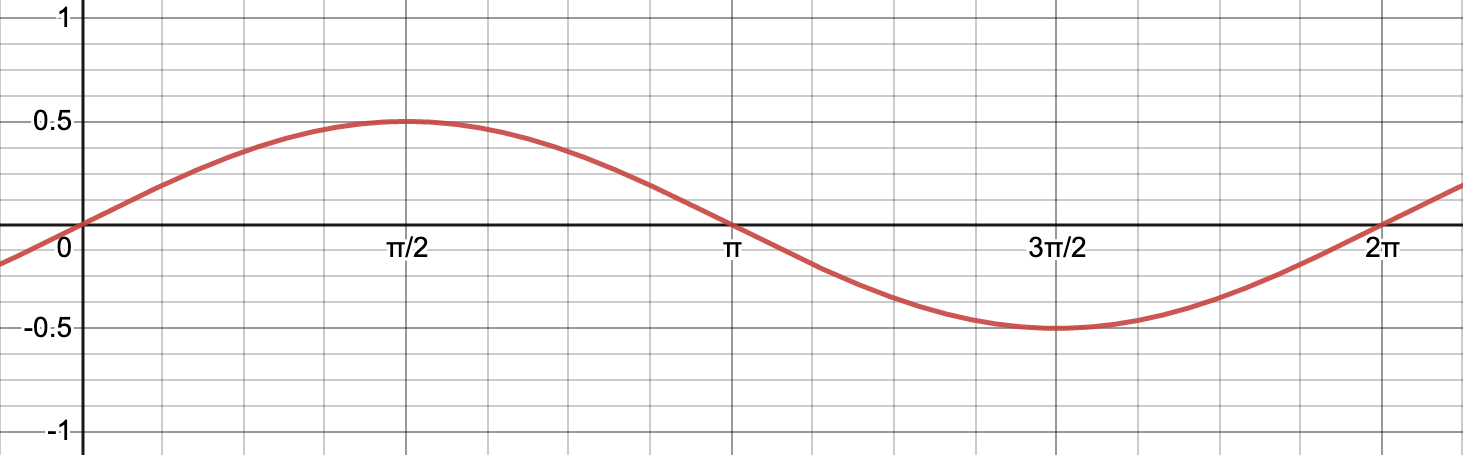
\includegraphics[width=\textwidth]{figures/half-sized-sine-wave.png}
	\caption{A sine wave, with an amplitude of $\frac{1}{2}$}
	\label{fig:half-sized-sine-wave}
\end{figure}

The second option commonly used to manipulate audio is to change an audio signal or wave's frequency. For sound and audio manipulations, the frequency component determines a sound's \say{color,} or \say{timbre.} It is the property of a waveform which determines the output sound's pitch. The high-end of audible frequencies for the human ear is around 20,000 Hz (20 kHz), though this reduces with age. The generally accepted range of human hearing ranges from 20 Hz to 20 kHz, with frequencies below 20 Hz felt more than heard\cite{Rosen_Howell_2011}. This range is further broken down in Table \ref{tbl:frequency-table-of-human-hearing-general}. Thus, with Equation \ref{eq:full-sine-wave-equation}, we change the value of $w$, which increases the rate of change of the sine wave, increasing the perceived pitch. With the period of the sine wave in Figure \ref{fig:sine-wave-period-amplitude} marked blue, it is this blue section that will increase with an increase in $\omega$. As $\omega$ increases, there are more repetitions of the sine wave's phase, so the audio output's pitch will increase. Pitch is how high or low a sound is perceived to be, and will be determined by the frequency of the vibrations \cite{Toft_2020}. Frequency is the number of wave cycles which pass through a given point per second. A higher frequency will result in a higher pitch, and a lower frequency will result in a lower pitch. For instance, with a frequency of 261 Hz, we perceive the note Middle C to be played. 

Finally, a modification to a wave's phase will determine if the audio signal output is on-time, delayed, or early. The numeric value of $\varphi$ depends on the start of the wave's period. Similar to the changes made to amplitude and frequency, by modifying the value of $\varphi$, we change the phase of the waveform. This will be most noticeable with multiple harmonics or simple waveforms stacked on top of each other, in which each signal will have a phase at a slightly different time, as in Figure \ref{fig:sine-wave-phase-shift}. The period of the blue sine wave has a length of $\frac{\pi}{2}$, but otherwise is a normal unit circle sine wave. The red sine wave is phase shifted, with an $\varphi$ value of positive 2, which shifts the wave negative and to the left, causing the output audio to sound early in comparison to the blue wave. 

\begin{figure}[ht]
	\centering
	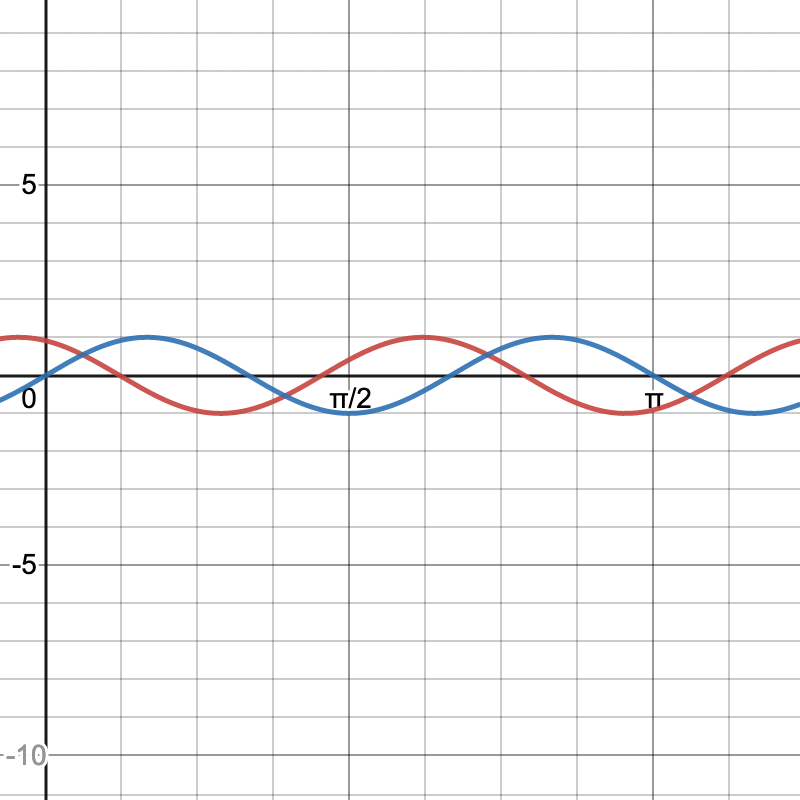
\includegraphics[width=0.5\textwidth]{figures/sine-wave-phase-shift.png}
	\caption{The phase shift in a sine wave}
	\label{fig:sine-wave-phase-shift}
\end{figure}


This type of sound modulation is done through this synthesizer's ``delay'' effect (sometimes known as ``echo'' effect). It is an effect which records an input signal, stores it, then plays it back after a defined time. Typically, the delayed audio is mixed with the live audio input creating an echo effect, where we first hear the original audio, followed by the delayed audio. The value of $D$ in Equation \ref{eq:sine-wave-equation} determines the shift of the wave, and thus also the sound. A positive value (such as $\frac{\pi}{2}$) will shift the sine wave to the left on the Cartesian plane, resulting in a sine wave which sounds early. The same applies to a negative $D$ value, in which a value such as $-\frac{\pi}{6}$ shifts the sine wave to the right, creating a sine wave which sounds ``late'' or delayed.

Other modules can be created through similar logic. To create legato and staccato, we either connect the waves of different frequencies together, or separate the waves to the point there is a clear distinction between the notes. Musically, these two concepts are total opposites; staccato is defined as the style of playing notes in a detached and separated manner, in which each note is clearly distinct from one another. It is typically indicated by a dot directly above or below the notehead, depending on if the stem of the note goes upwards (a dot is placed below the notehead), or goes downwards (a dot is placed above the notehead) \cite{Burkholder_Grout_Palisca_2014}. An example of staccato is in Figure \ref{fig:bartok-dance-five-b-section}, in which there are dots clearly above and below some of the notes, and the location of the dot is dependent on whether the stems of the notes face upwards or downwards. Legato is the directive which defines notes to be played in a smooth and connected manner, with notes that are no longer clearly distinctive from one another, as each note will flow gracefully into the next.

\begin{figure}[h]
  \centering
  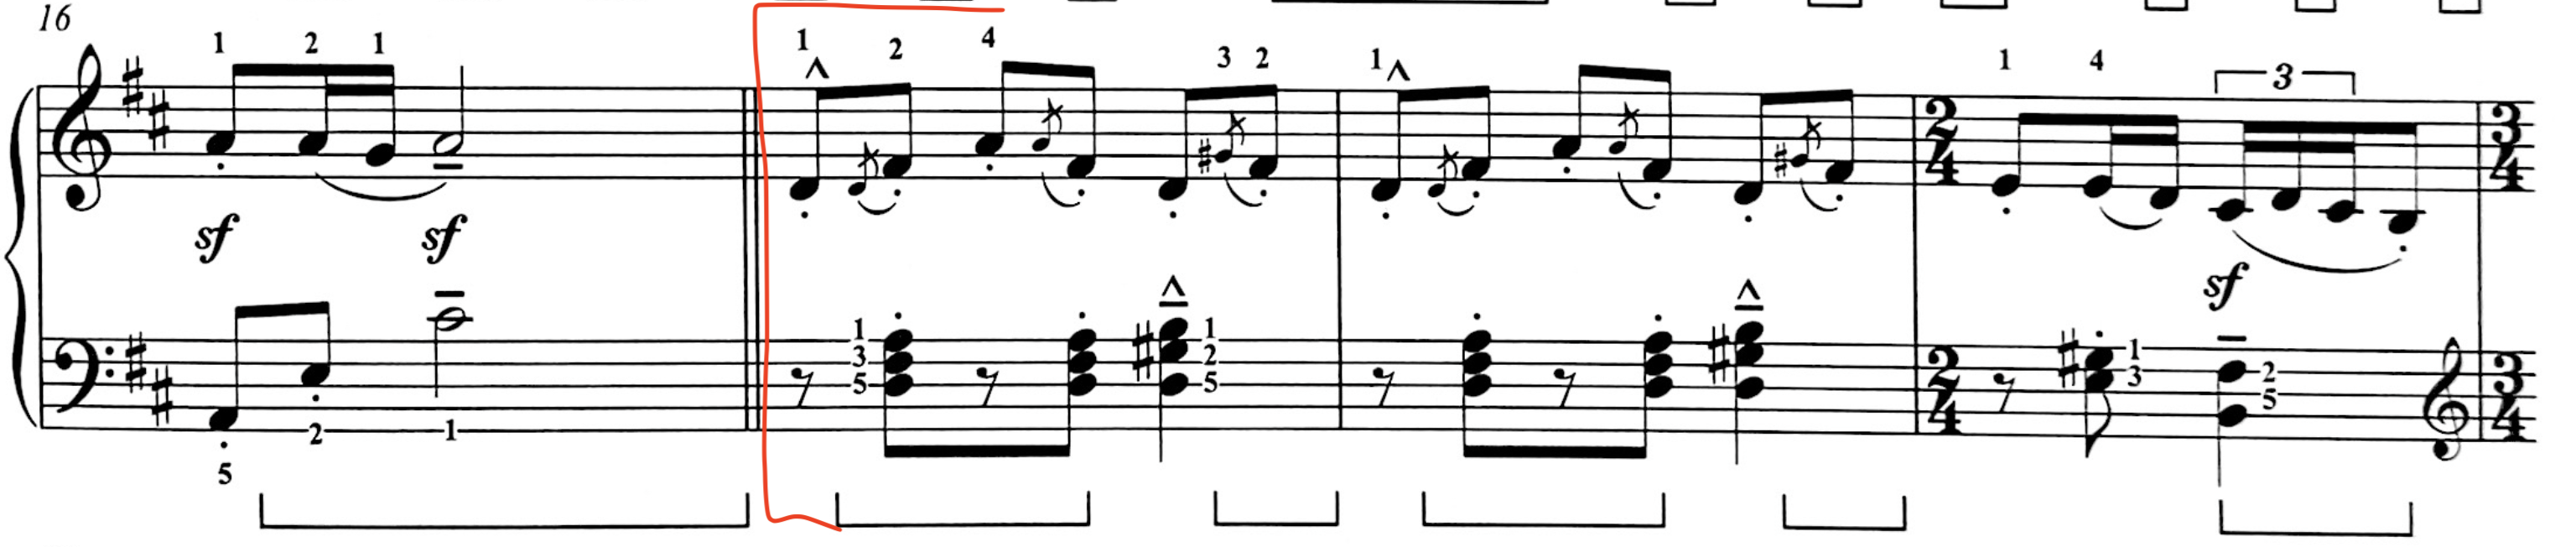
\includegraphics[width=\textwidth]{bartok-dance-five-b-section.jpg}
  \caption{Béla Bartók, Romanian Folk Dances, \textit{Poarga Românească}, mm. 16-19}
  \label{fig:bartok-dance-five-b-section}
\end{figure}

We will also create a module meant to layer specific harmonics over a base frequency: the major third interval, and the perfect fifth interval, which together will form a major chord. A chord can be defined as the simultaneous sounding of two or more notes (typically three or more). Most chords are triadic in nature (that is, containing only three notes), with the interval of a major third or minor third between each of the three notes. The major third interval can be defined as the interval which spans four degrees of the diatonic scale in the Western twelve-semitone tuning system (refer to subsection \ref{subsection:how-midi}), or four semitones \cite{Nave_2017}.\footnote{The major third interval is also enharmonically equivalent to the diminished fourth interval. The enharmonic interval describes notes which sonically are the same, yet notated differently.} The minor third interval contains one fewer degrees than the major third interval, thus having only two degrees of the diatonic scale, and so only three semitones. For instance, the interval between $A$ and $C\musSharp{}$ is a major third, as the note $C\musSharp{}$ lies four semitones away from the note $A$, while the interval between $A$ and $C$ is a minor third, with the note $C$ lying only three semitones away from the note $A$. Notable examples of the major third interval include the first two notes of the song ``When the Saints Go Marching In,'' the first movement of Ludwig van Beethoven's \textit{Fifth Symphony} (Figure \ref{fig:beethoven-fifth} \cite{Beethoven_1862}), or the song ``Swing Low, Sweet Chariot.'' Examples of the minor third interval include the first two notes of the tune of ``Greensleeves,'' (Figure \ref{fig:greensleeves} \cite{Kurtz_2010}) Christmas tune ``What Child is This,'' or The Beatles' ``Hey, Jude.''

\begin{figure}[ht]
  \centering
  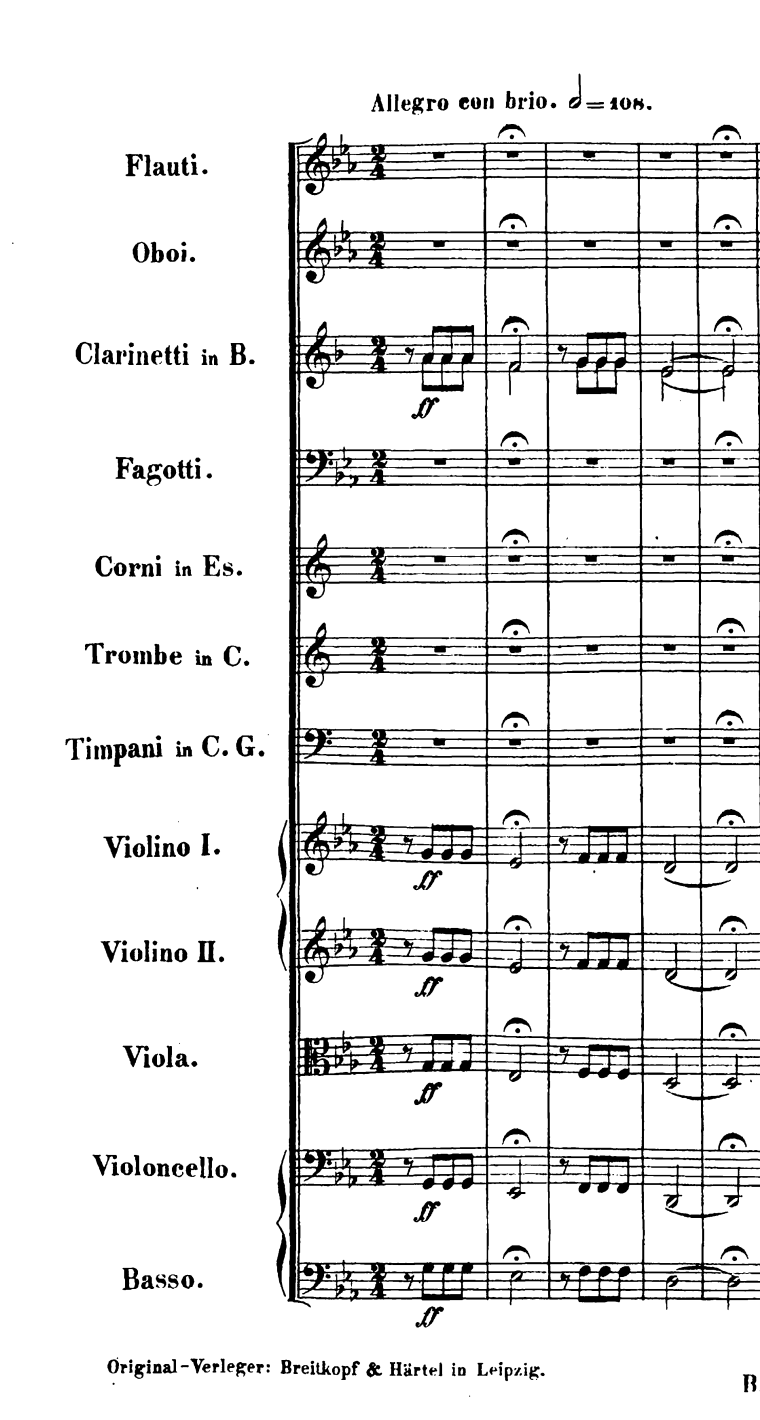
\includegraphics[width=0.5\textwidth]{beethoven-fifth.jpg}
  \caption{Ludwig van Beethoven, Symphony No. 5 in C Minor, \textit{Allegro con brio}, mm. 1-4}
  \label{fig:beethoven-fifth}
\end{figure}

\begin{figure}[ht]
  \centering
  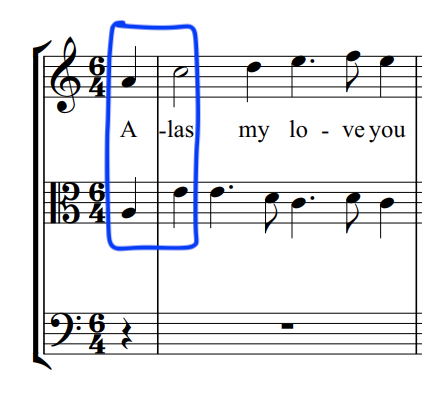
\includegraphics[width=0.4\textwidth]{greensleeves.jpg}
  \caption{``Greensleeves'', mm. 1}
  \label{fig:greensleeves}
\end{figure}

The interval of the third is important to distinguish \textit{major} chords, and \textit{minor} chords, as major chords will have a root note (the tonic note), major third interval, and another minor third interval (or perfect fifth interval above the tonic) stacked on top of one another, while a minor chord will have the tonic, minor third, and perfect fifth. Either multiple waveforms (of the specified major third and perfect fifth intervals) can be stacked to produce the major chord sound, or MIDI inputs can trigger a major chord.

To add the distortion alteration (as opposed to the specific distortion effect) to a sound is simply to add desired textures to a sound, through changing and deforming an audio signal's waveform. For many, a prime example is seen with the use of an electric guitar, as the pedals used with an electric guitar allow for added harmonics, and other changes made to the guitar's sound. One of the most used types of distortion is known as \textit{clipping}, in which the level of a signal (typically amplitude) goes beyond the maximum that a system is able to handle, leading to clipping, as the maximum of the waveforms gets abruptly cut off at the system's maximum. At its best form, distortion can be a gentle audio effect, which can add many types of sounds to a signal, including saturating the sound, and adding overdrive and \textit{fuzz} through adding \textit{gain} (defined as an increase in some type of value). Within the field of distortion, \textit{gain} is referred to as \textit{transmission gain}, in which there is an increase in the power of a signal, expressed in \textit{decibels} (dB), usually done through an arbitrary combination of increasing the amplitude and frequency of a sound wave.

The two most common, and most subtle, types of distortion are saturation and clipping. The result of these two types of clipping is ``soft clipping'' in which the peaks of the signal's waveform are softly rounded, and not abruptly cut off \cite{Tarr_2019}. The signal will be pushed only slightly over the 0 dB threshold. 

The concept of the 0 dB threshold is important, as it is a fundamental aspect of music production and mixing, as well as how to effectively create distortion within a modular synthesizer. Both digital and analog meters for volume, as in Figure \ref{fig:server-meter}, have ranges between negative infinity (or silence), up to 0 dB (the absolute loudest). These decibels are different that the standard decibels used to describe the loudness of everyday sounds. Standard decibels allow us to compare the relative loudness of sounds to each other; a jet taking off sounds at 140 dB, a firecracker is 140-165 dB, and a whisper may be 30 dB \cite{Hearing_Health_Foundation}. These decibels act as a unit measurement for sound, and the National Institute of Occupational Safety (NIOSH) states that while exposure to noise at 85 decibels or above  will cause hearing loss, the exposure dangers for higher levels become exponentially more damaging. While at a noise level of 70 dB would take over 24 hours to cause hearing damage, sound at a level of 115 dB would cause hearing damage at only 28 seconds. The 115 dB volume of a rock concert and symphonic orchestra concert is much more noticeable, especially when comparing to the volume of listening to music on personal devices at maximum volume (105 dB).

The type of decibels used for music production are ``Decibels Full Scale'' (dBFS) when discussing digital music, or ``Sound Pressure Level'' (dB SPL) in the real world. This is the measurement of decibels as it pertains to the levels in an audio recording. Unlike the scale for dB, in which 0 dB is absolute silence, and higher numbers indicate a louder perceived volume, the scale for dBFS is reversed. With the dBFS scale, 0 dB is the maximum level of audio a system can process before it ``clips'' the signal. The lowest detectable level of sound in the system, the ``noise floor,''  can be as low as -150 dB, but is typically between -80 dB and -90 dB. In general, the common range for volume lies between -10 and -18 dB, leaving 10 dB as headroom when combining all audio signals into one master track.

\begin{figure}
  \centering
  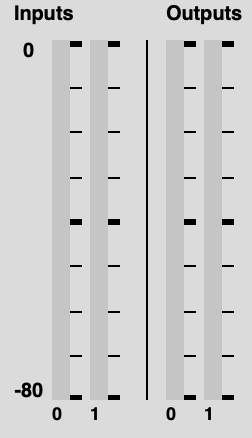
\includegraphics[width=0.2\textwidth]{server-meter.jpg}
  \caption{The server meter in SuperCollider}
  \label{fig:server-meter}
\end{figure}

So, keeping the noise level somewhere between -80 dB and -10 dB will help in introducing distortion to pure sound waveforms. If a signal is ``softly clipped'' (boosted slightly over the 0 dB threshold), the output sound may contain subtle harmonics (other frequencies overlaid on top of the original frequency) or other overtones. 

Overdrive, the distortion effect, and fuzz are three other types of distortion effects, and now are synonymous with electric guitar rigs, pedals, and other similar hardware. Overdrive tends to be the most subtle of the three, with higher gain levels. Distortion and fuzz are more intense, with distortion allowing for large amounts of sustain, harmonics, and a mostly altered sound from the original input, noticeable in heavy rock music and guitar solos. Fuzz is similar to distortion in gain level, but also employs the use of a \textit{frequency multiplier} to produce sound similar to that of a square wave. Distortion using the fuzz effect produces a traditional synth-like effect, with digital artifacts, or overly processed sounds.
